\documentclass{article}
\usepackage[utf8]{inputenc}
\usepackage{graphicx}
\usepackage{caption}
\usepackage{minted}





\title{Relazione progetto GPU computing}
\author{Martino Tiziani}
\date{Maggio 2019}

\begin{document}

\maketitle

\section{Attacco Algebrico}

Un'attacco algebrico è un particolare tipo di attacco crittografico che fa uso dell'algebra lineare per attaccare un cifrario. La tecnica si compone di due fasi:

\begin{itemize}
\item \textbf{fase di traduzione}: si effettua una traduzione del cifrario, che deve essere attaccato, in un sistema di equazioni polinomiali con coefficienti in un campo finito (il modulo è quindi un numero primo).

\item \textbf{fase di risoluzione}: si risolve il sistema di equazioni, appena trovato, e si estrae dalla soluzione la chiave segreta del cifrario originale (o parte di essa).

\end{itemize}

Questo attacco è molto interessante per via della sua versatilità, infatti questa tecnica è applicabile a tutti i cifrari che sono scrivibili come un sistema di equazioni, la grande potenzialità è che tutti i cifrari realizzati fino ad oggi possiedono questa proprietà. 

L'attacco algebrico risulta quindi un attacco che può essere utilizzato su qualsiasi cifrario, tuttavia è ancora poco conosciuto, rispetto ad altre tecniche di crittoanalisi e questo è dovuto alla sua complessità computazionale. Infatti senza entrare troppo nel dettaglio nella teoria della complessità la fase di risoluzione di un sistema di equazioni lineari in campo finito è classificato come NP-complete. Un problema con questa complessità risulta irrisolvibile, in un tempo accettabile, per istanze di grosse dimensioni, e anche con piccole dimensioni i tempi di esecuzione sono elevati. Tuttavia il parallelismo potrebbe portare in alcuni casi dei benefici da non sottovalutare.

\section{Risolvere il sistema}

Risolvere il sistema di equazioni che descrive il cifrario in discussione è il punto centrale dell'attacco algebrico. Esistono diverse tecniche per risolvere tale sistema, alcune banali altre più ricercate e complesse. Molte di queste tecniche hanno benefici su particolari istanze di problema o in determinate condizioni. Il meccanismo di risoluzione qui esposto (realizzato come lavoro di tesi triennale) si compone di due fasi: 

\begin{itemize}
\item \textbf{fase di espansione}: si espande il sistema aggiungendo delle equazioni in modo tale che il sistema risulti risolvibile.
\item \textbf{fase di riduzione}: si riduce il sistema di equazioni con l'algoritmo di eliminazione di Gauss (si eliminano le equazioni linearmente dipendenti).

\end{itemize}

Si ripetono queste fasi fino alla soluzione completa del sistema (trovare i valori delle incognite delle equazioni). La fase di espansione è necessaria perché il sistema di partenza non è, quasi mai, direttamente risolvibile, ovvero non possiede sufficienti equazioni per poterne determinare la soluzione.

\section{Riduzione di Gauss e parallelismo}

Il fulcro di tutta la tecnica realizzata è la riduzione di Gauss di un sistema di equazioni modulari. Questo algoritmo rappresenta il sistema sotto forma di una matrice (monomi delle equazioni ordinati secondo un preciso ordinamento, in questo caso: \textit{grevlex}) e ripete su di essa un set di operazioni consentite.
\begin{itemize}
\item scambiare due righe
\item moltiplicare una riga per un numero diverso da zero
\item sommare alla riga il multiplo di un'altra riga
\end{itemize}

Lo scopo dell'algoritmo è trasformare la matrice di partenza in una matrice a scalini. Ottenuta questa forma il sistema può essere facilmente risolto per sostituzione inversa.

	\begin{center}
		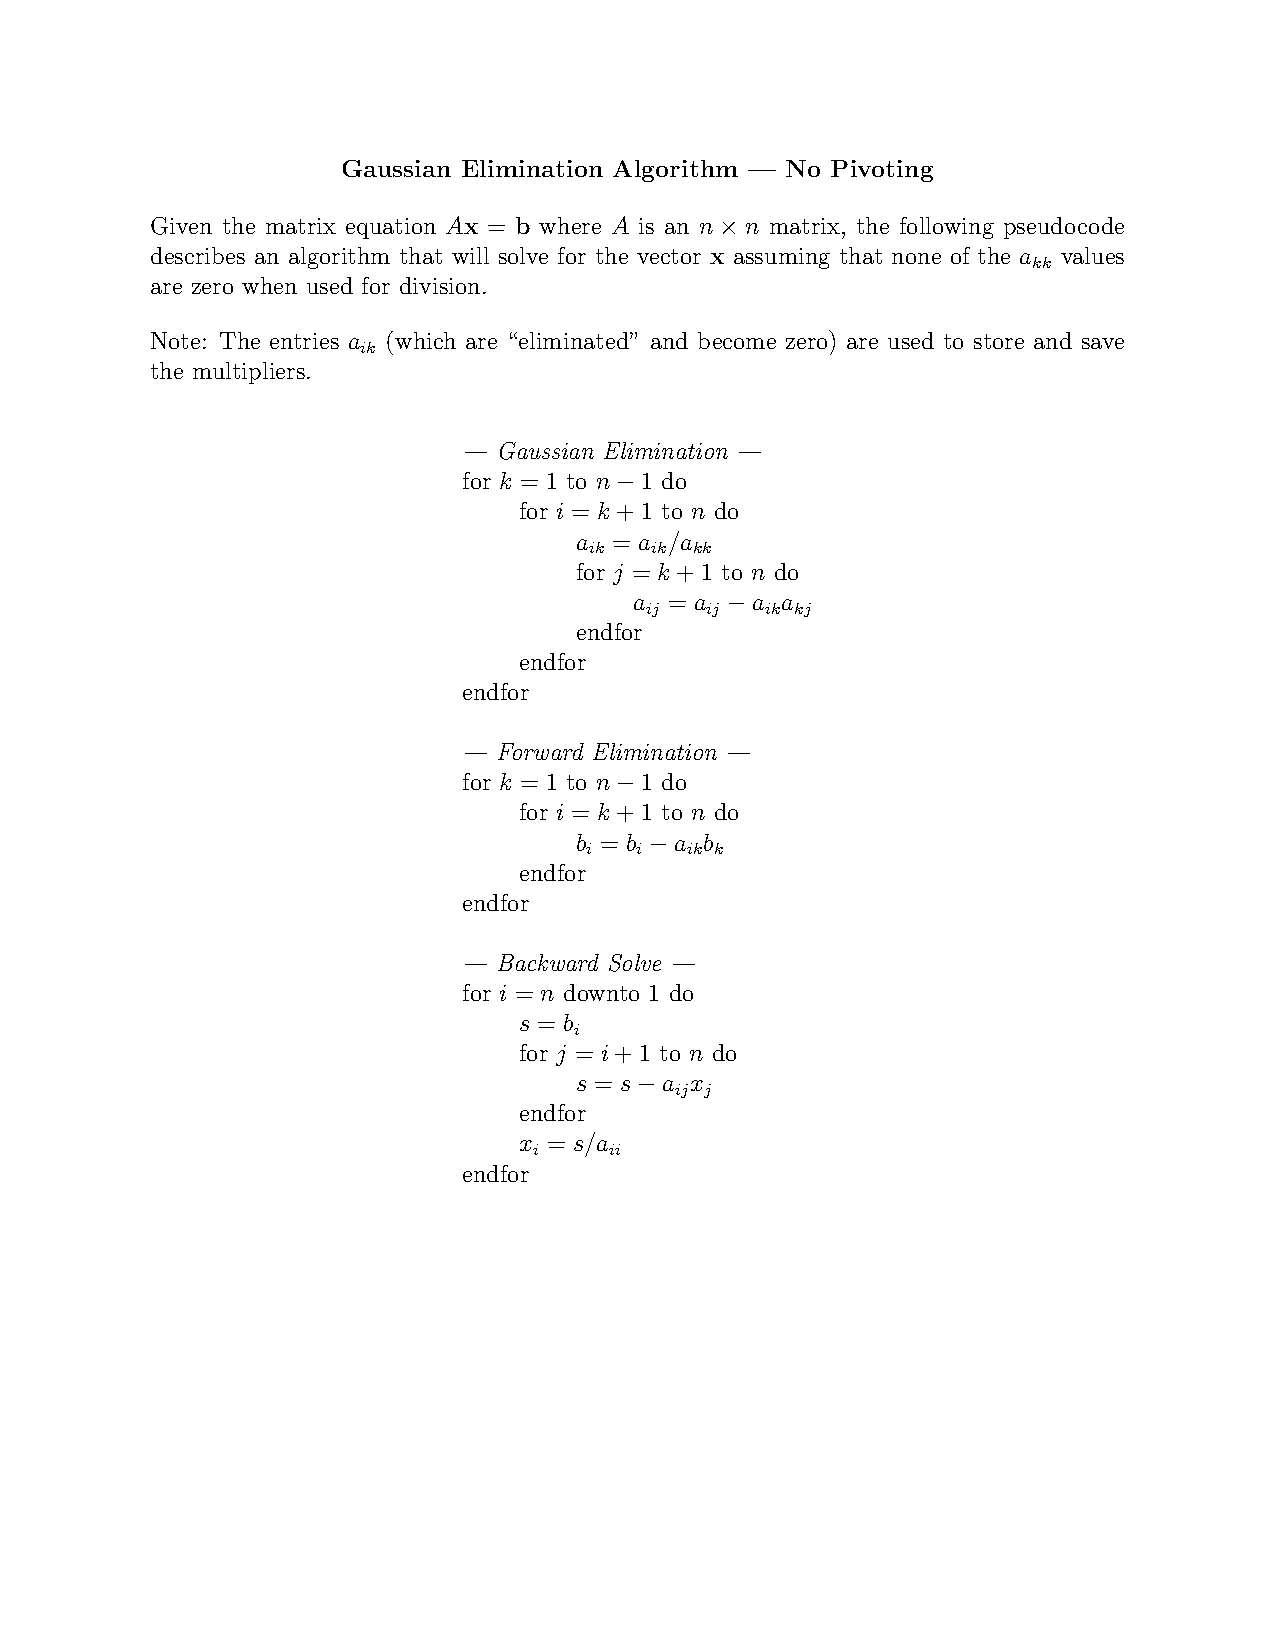
\includegraphics[width = \textwidth]{gauss.png}
		\captionof{figure}{Riduzione a scalini della matrice}
		\label{fig:gauss}
	\end{center}

Fortunatamente questo algoritmo è per sua natura parzialmente parallelizzabile. Ci sono diverse varianti di questo algoritmo, qui viene utilizzata la riduzione di Gauss con pivot completo. Come da pseudocodice si nota che i due cicli interni effettuano operazioni completamente indipendenti su dati indipendenti, percio tali operazioni possono essere eseguite completamente in parallelo. Nella realizzazione del sistema si è sfruttato il parallelismo su CPU per velocizzare il più possibile la computazione, tuttavia data la natura fortemente parallela di una porzione dell'algoritmo è senza dubbio interessante verificare come il parallelismo di una GPU possa influenzare tale computazione.

\section{Implementazione CUDA}

Come detto in precedenza esistono tanti metodi per risolvere il sistema di equazioni in esame. La riduzione di Gauss è senza dubbio uno dei metodi più banali, tuttavia fornisce al programma una generalità (non sfrutta nessuna condizione specifica, funziona sempre) che le altre tecniche non forniscono. La stessa riduzione di Gauss può essere effettuata in diversi modi, ciononostante lo scopo di questo progetto è quello di comparare l'implementazione parallela realizzata su CPU con quella per GPU, per cui non vengono utilizzate diverse risoluzioni come ad esempio la decomposizione LU, o altre.

Il problema e gli elementi su cui bisogna lavorare sono espressi più chiaramente dalla Figura \ref{fig:mat}, gli scalini vengono generati in senso opposto rispetto alla normale riduzione di Gauss a causa dell'ordinamento utilizzato. Si noti che, dopo aver identificato una colonna e riga pivot (celle arancione), deve essere ridotta tutta la sottomatrice (di colore giallo) sottostante il pivot, per ottenere l'i-esimo scalino (colonna pivot ridotta a 0 a partire dalla riga sottostante il pivot). La riduzione di questa porzione di matrice può avvenire in modo completamente parallelo.

	\begin{center}
		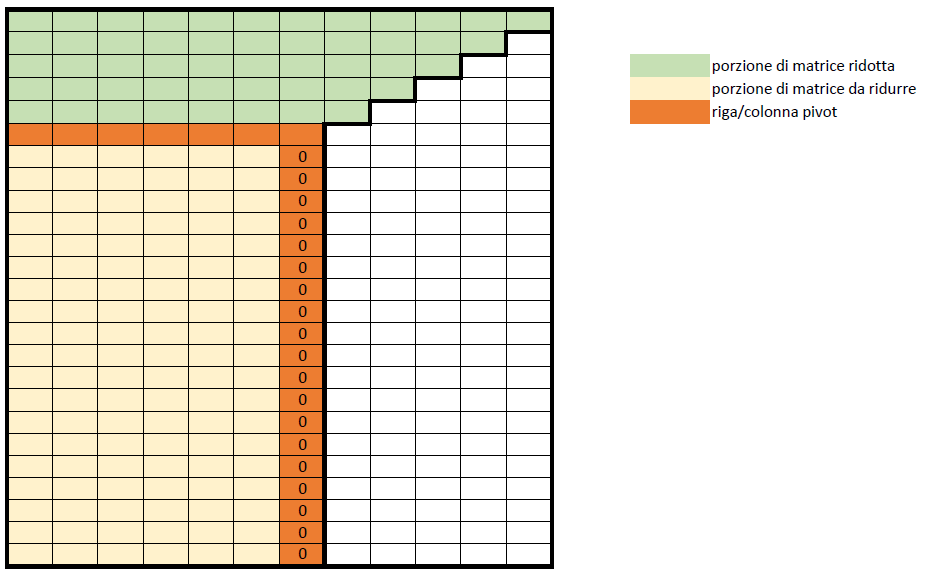
\includegraphics[width = \textwidth]{matrice.png}
		\captionof{figure}{Schema della struttura della matrice}
		\label{fig:mat}
	\end{center}


Sono state realizzate tre tecniche per ridurre la porzione di matrice gialla:
\begin{itemize}
\item \textbf{celle}: il kernel effettua la riduzione di una sola cella
\item \textbf{righe}: il kernel effettua la riduzione di una riga 
\item \textbf{blocco}: il kernel effettua la riduzione di un blocco della colonna
\end{itemize}

\newpage
Prima di procedere oltre è necessario riflettere su come implementare il ciclo esterno, tale operazione infatti non è parallelizzabile. Si possono adottare due scelte:
\begin{itemize}
\item effettuare il ciclo esterno su CPU in modo veloce ed efficiente per poi trasferire su GPU la matrice e risolvere la riduzione in parallelo.
\item effettuare il ciclo esterno su un singolo kernel in modo poco efficiente e sfruttare il \textbf{parallelismo dinamico} per lanciare la riduzione successiva.
\end{itemize}

La prima tecnica per quanto possa sembrare appetibile non è utilizzabile, in quanto il numero di trasferimenti della matrice risulta essere troppo elevato, quando la dimensione della matrice inizia a crescere i trasferimenti diventano insostenibili. La seconda tecnica sacrifica le performance del ciclo esterno per mantenere la matrice sempre in memoria globale della GPU evitando continui e costosissimi trasferimenti di memoria con la CPU. Per tanto si sono realizzate le tre tecniche precedenti sfruttando il parallelismo dinamico.

\section{Risultati preliminari}
Di seguito si forniscono i risultati ottenuti con una prima implementazione, che non sfrutta alcun tipo di ottimizzazione, delle tre tecniche descritte precedentemente. Gli input si riferiscono a dei sistemi di equazioni studiati appositamente per questo progetto. Tali sistemi si possono trovare nella directory \textit{input} del progetto, mentre nella Tabella \ref{table:2} si può trovare un riassunto delle loro proprietà principali. Non è possibile conoscere a priori la dimensione raggiunta dal sistema durante la procedura, le dimensioni riportate sono quindi una approssimazione della dimensione massima raggiunta. 

\begin{table}[h!]
\centering
 \begin{tabular}{|c | c | c | c |} 
 \hline
 Sistema & Grado & modulo & Dimensione matrice (MB)\\
 \hline
A & 8  & 1033   & 0.60\\
E & 11 & 5813   & 5.26\\	
H & 13 & 11927  & 12.66\\
G & 14 & 12437  & 21.60 \\
J & 16 & 21013  & 44.56\\
I & 18 & 32353  & 91.54\\
K & 20 & 49069  & 171\\
L & 22 & 60101  & 292\\
M & 27 & 117881 & 979\\
N & 27 & 128341 & 979\\
O & 29 & 153247 & 1493\\
P & 29 & 163199 & 1493\\
 \hline

\end{tabular}
\caption{Proprietà dei sistemi di input}
\label{table:2}
\end{table}
Di seguito i tempi di esecuzione su una Nvidia GTX 960.
\begin{table}[h!]
\centering
 \begin{tabular}{|c | c | c | c | c|} 
 \hline
 Sistema & CPU & celle & righe & blocco\\
 \hline
A & 0,0669    & 0,2110   & 0,2400   & 0,2650\\
E & 0,6487    & 0,3880   & 0,5550   & 0,5680\\	
H & 3,17      & 1,11     & 1,52     & 1,44\\
G & 6,07      & 1,63     & 1,91     & 1,80\\
J & 17,55     & 4,45     & 4,82     & 4,20\\
I & 52,36     & 11,46    & 11,66    & 9,78\\
K & 169       & 32       & 30       & 25\\
L & 303       & 58       & 48       & 42\\
M & 2086      & 363      & 268      & 233\\
N & 2292      & 406      & 299      & 264\\
O & 4083      & 710      & 483      & 439\\
P & 4520      & 786      & 548      & 492\\
 \hline

\end{tabular}
\caption{Tempi di esecuzione in secondi}
\label{table:1}
\end{table}


Come ci si aspettava l'esecuzione su GPU risulta essere più veloce di quella su CPU. Tuttavia si nota anche una grossa differenza tra le tre tecniche realizzate. In particolare si evince subito che utilizzare un kernel per ogni cella da ridurre risulta essere uno spreco a causa dell'overhead, ed all'aumentare della dimensione degli esempi questo problema non fa altro che aumentare. Di conseguenza questa tecnica non risulta adatta per questa computazione. Le altre due, invece, si prestano bene ad ottimizzazioni volte a diminuire i tempi di esecuzione.

\subsection{Profiling}
I primi risultati sono incoraggianti, le tecniche: righe e blocco forniscono buone prestazioni. A questo punto si cerca di ottimizzare il più possibile il kernel padre che lancia la riduzione tramite kernel figlio. Tale kernel infatti deve eseguire un numero considerevole di operazioni oltre che la riduzione: trovare il pivot, scambiare righe della matrice ed azzerare la colonna pivot. 
	\begin{center}
		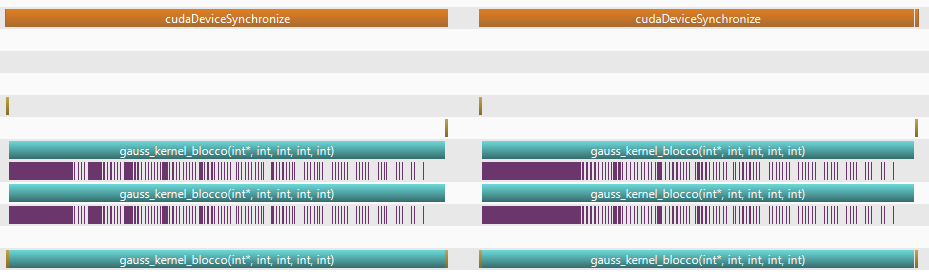
\includegraphics[width = \textwidth]{profiling.png}
		\captionof{figure}{Profiling della versione preliminare della tecnica blocco}
		\label{fig:profiling}
	\end{center}
	
Come si nota dalla Figura \ref{fig:profiling} e dalla sessione di profiling, nella directory \textit{profiling}, il kernel (figlio) che effettua la riduzione della sottomatrice occupa solo una porzione relativamente piccola del kernel padre (circa 25\%), questo è visibile anche dagli "spazi bianchi" della figura. Questo indica che molto tempo è perso dal kernel padre per effettuare altre operazioni necessarie. Come detto in precedenza esiste \textbf{un solo kernel padre}, quindi tutte le operazioni non effettuate tramite parallelismo dinamico risultano essere eseguite serialmente. La prima ottimizzazione necessaria è quindi senza dubbio effettuare queste operazioni tramite kernel figli.

\section{Ottimizzazioni (shared memory - parallelismo dinamico)}
\paragraph{Parallelismo Dinamico} dal profiling si evince che è necessario effettuare ulteriori operazioni (trovare il pivot, scambiare righe della matrice, azzerare la colonna pivot) tramite parallelismo dinamico. Si realizzano quindi i kernel necessari per tali operazioni. Si sposta cosi il carico di lavoro dal kernel padre ai figli, a questo punto il padre non effettua più molto lavoro, si preoccupa solo di iterare sulle varie colonne della matrice e lanciare le operazioni necessarie tramite parallelismo dinamico. Il parallelismo dinamico introduce purtroppo del ritardo nella computazione, infatti quando un kernel padre lancia kernel figli deve attendere il completamento di questi tramite \mintinline{cuda}{cudaDeviceSynchronize()}. I kernel delle diverse operazioni hanno bisogno della loro sincronizzazione, per cui all'aumentare del numero di operazioni effettuate, tramite parallelismo dinamico, aumenta l'overhead di sincronizzazione. 

\paragraph{Shared Memory} un'ulteriore ottimizzazione è senza dubbio l'utilizzo della shared memory, che in questo caso è di enorme aiuto per mantenere informazioni sul pivot. Come indicato dallo pseudocodice è necessario conoscere il valore di tutta la riga pivot per effettuare la riduzione della sottomatrice. Ad ogni cella non-nulla della sottomatrice si sottrae un valore multiplo della riga pivot, per cui poter accedere velocemente ed efficientemente a queste informazioni è fondamentale per le prestazioni dell'intero programma.

Per il kernel righe si può utilizzare la shared maemory per contenere la riga pivot. Per il kernel blocco si può utilizzare la shared memory in maniera migliore, si memorizza infatti una porzione sia della riga pivot che della colonna pivot. 

\section{Risultati finali}
Di seguito si riportano le performance del programma sfruttando le ottimizzazioni precedentemente descritte.

\begin{table}[h!]
\centering
 \begin{tabular}{|c | c | c | c |} 
 \hline
 Sistema & CPU & righe & blocco\\
 \hline
A & 0,0669    & 0.223 & 0.251\\
E & 0,6487    & 0.406 & 0.435\\	
H & 3,17      & 0.957 & 0.866\\
G & 6,07      & 1.209 & 1\\
J & 17,55     & 2.80  & 1.90\\
I & 52,36     & 6.44  & 3.75\\
K & 169       & 17    & 8\\
L & 303       & 27    & 14\\
M & 2086      & 181   & 93\\
N & 2292      & 195   & 103\\
O & 4083      & 345   & 183\\
P & 4520      & 384   & 202\\
 \hline

\end{tabular}
\caption{Tempi di esecuzione in secondi}
\label{table:1}
\end{table}

\subsection{profiling}
Si nota subito sia dai risultati ottenuti in che dalla Figura \ref{fig:profiling_optimized} come l'utilizzo di più kernel e shared memory aumenta l'efficienza e riduce notevolmente i tempi di esecuzione. 
	\begin{center}
		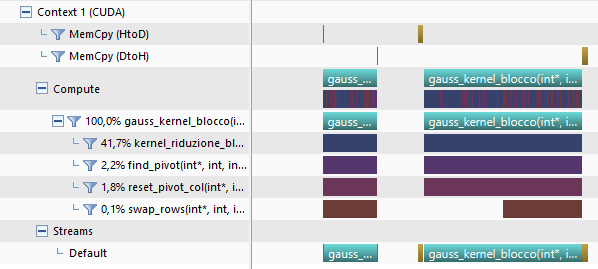
\includegraphics[width = \textwidth]{profiling_optimized.png}
		\captionof{figure}{Profiling della versione ottimizzata della tecnica blocco}
		\label{fig:profiling_optimized}
	\end{center}



\section{Considerazioni finali}
E' evidente che l'utilizzo della GPU comporta prestazioni molto più elevate rispetto alla CPU. Il forte parallelismo di una porzione dell'agloritmo di eliminazione di Gauss permette di sfruttare appieno le potenzialità delle moderne GPU. D seguito si presenta un confronto grafico della prestazione CPU-GPU, si noti che i risultati della GPU sono stati ottenuti con un hardware di basso livello, l'utilizzo di schede apposito può portare sicuramente a prestazioni molto più elevate.


\end{document}